\psfrag{O}[c][c] {$\mathcal{O}$}
\psfrag{R2}[c][c] {$\mathbb{R}^2$}

\psfrag{mn}[c][c] {$-$}
\psfrag{pl}[c][c] {$+$}

\psfrag{c}[c][c] {$c$}

\psfrag{x}[c][c] {$x$}
\psfrag{y}[c][c] {$y$}
\psfrag{sxi}[c][c] {$\sigma_{\xi\xi}$}
\psfrag{seta}[c][c] {$\sigma_{\eta\eta}$}
\psfrag{sxieta}[c][c] {$\sigma_{\xi\eta}$}

\psfrag{p0}[c][c] {$0\pi$}
\psfrag{p1}[c][c] {$\frac{\pi}{12}$}
\psfrag{p2}[c][c] {$\frac{\pi}{6}$}
\psfrag{p3}[c][c] {$\frac{\pi}{4}$}
\psfrag{p4}[c][c] {$\frac{\pi}{3}$}
\psfrag{p5}[c][c] {$\frac{5\pi}{12}$}
\psfrag{p6}[c][c] {$\frac{\pi}{2}$}
\psfrag{p7}[c][c] {$\frac{7\pi}{12}$}
\psfrag{p8}[c][c] {$\frac{2\pi}{3}$}
\psfrag{p9}[c][c] {$\frac{3\pi}{4}$}
\psfrag{p10}[c][c] {$\frac{5\pi}{6}$}
\psfrag{p11}[c][c] {$\frac{11\pi}{12}$}
\psfrag{p12}[c][c] {$\pi$}
\psfrag{p13}[c][c] {$\frac{13\pi}{12}$}
\psfrag{p14}[c][c] {$\frac{7\pi}{6}$}
\psfrag{p15}[c][c] {$\frac{5\pi}{4}$}
\psfrag{p16}[c][c] {$\frac{4\pi}{3}$}
\psfrag{p17}[c][c] {$\frac{17\pi}{12}$}
\psfrag{p18}[c][c] {$\frac{3\pi}{2}$}
\psfrag{p19}[c][c] {$\frac{19\pi}{12}$}
\psfrag{p20}[c][c] {$\frac{5\pi}{3}$}
\psfrag{p21}[c][c] {$\frac{7\pi}{4}$}
\psfrag{p22}[c][c] {$\frac{11\pi}{6}$}
\psfrag{p23}[c][c] {$\frac{23\pi}{12}$}
\psfrag{p24}[c][c] {$2\pi$}

\psfrag{x1}[c][c] {$x_1$}
\psfrag{x2}[c][c] {$x_2$}

\psfrag{imz}[c][c] {$\Im(z)$}
\psfrag{rlz}[c][c] {$\Re(z)$}

\psfrag{c}[c][c] {$c$}
\psfrag{acr}[c][c] {$\textsc{\tiny Crevice }$}
\psfrag{nuc}[c][c] {$\textsc{\tiny Nucleation}$}
\psfrag{a}[c][c] {$a$}
\psfrag{fa}[c][c] {$\mathfrak{f} (a)$}
\psfrag{aabs}[c][c] {$\| a \|$}
\psfrag{b}[c][c] {$b_{\epsilon \ll 1}$}
\psfrag{p0}[c][c] {$p_{h}$}

\psfrag{sost}[c][c] {$\textsc{\tiny Solid-state}$}
\psfrag{sse}[c][c] {$\textsc{\tiny Polycrystalline}$}
\psfrag{ese}[c][c] {$\textsc{\tiny electrolyte}$}

\psfrag{sdd}[c][c] {$\textsc{\tiny Dendritic}$}
\psfrag{itf}[c][c] {$\textsc{\tiny Interface}$}

\psfrag{an}[c][c] {$\textsc{\tiny Anodic}$}
\psfrag{ca}[c][c] {$\textsc{\tiny Cathodic}$}
\psfrag{elt}[c][c] {$\textsc{\tiny Electrode}$}

\psfrag{iaw}[c][c] {$\WABsigma \xrightarrow[(ii)]{z\rightarrow\infty} 0$}
\psfrag{naw}[c][c] {$\WABsigma \xrightarrow[(i)]{z\rightarrow 0} (-p_{h})$}

\psfrag{dd}[c][c] {$\textsc{Dendritic}$}
\psfrag{anel}[c][c] {$\textsc{Space charge layer } \cite{Braun2015}$}

\psfrag{mi}[c][c] {$\textsc{Mesoscopic}$}
\psfrag{mc}[c][c] {$\textsc{Prescribed crevice}$}

\psfrag{psr}[c][c] {$\textsc{\tiny Prescribed}$}
\psfrag{cr}[c][c] {$\textsc{\tiny Crevice/Crack}$}
\psfrag{len}[c][c] {$\textsc{\tiny Length } a$}

\psfrag{aw}[c][c] {$\textsc{Airy-Westergaard}$}
\psfrag{bc}[c][c] {$\textsc{Boundary conditions}$}

\psfrag{sca}[c][c] {$\textsc{Length scale } \left[m\right]$}
\psfrag{sma}[c][c] {$\textsc{Macro }$}
\psfrag{sme}[c][c] {$\textsc{Meso }$}
\psfrag{smi}[c][c] {$\textsc{Micro }$}

\psfrag{mls}[l][l] {$\textsc{\tiny \textbf{M}-like shape }$}
\psfrag{act}[l][l] {$\textsc{\tiny at crack tip }$}
\psfrag{acv}[l][l] {$\textsc{\tiny along grain boundary }$}

\psfrag{assb}[c][c] {$\textsc{All-solid-state Batteries }$}
\psfrag{abr}[c][c] {$\textsc{(ASSBs)}$}

\psfrag{bkn}[c][c] {\faChainBroken}

\psfrag{rt1}[c][c] {$\textsc{Routine 1}$}
\psfrag{rt2}[c][c] {$\textsc{Routine 2}$}
\psfrag{rt3}[c][c] {$\textsc{Routine 3}$}

\psfrag{eq1}[c][c] {$\displaystyle \frac{\partial \Bu}{\partial t} +  \nabla\cdot(\Bu\Bu) - \nabla\cdot(\nu\nabla\Bu) = -\nabla p$}
\psfrag{eq2}[c][c] {$\nabla\cdot\Bu=0$}

\psfrag{eq3}[c][c] {$\nabla \cdot
	(
	\accentset{\tiny 4}{\mbC}^{f^{\mcD(\Omega)}_{(\lambda,\mu)}}
	:
	\accentset{\tiny 2}{\overline{\nabla\Bu}}^{(s)}
	)
	= -\rho\,\nabla V_{e}
	%------------------------------------------
	\xrightarrow
	[
	\Bvarepsilon_{(E,\nu)}=
	\accentset{\tiny 2}{\overline{\nabla\Bu}}^{(s)}
	]
	{
	\accentset{\tiny 4}{\mbC}^{f^{\mcD(\Omega)}_{(\lambda,\mu)}}
	\to
	\accentset{\tiny 0}{\textbf{E}}:=E
	% E
	}
	E
	\nabla \cdot
	% \accentset{\tiny 0}{\textbf{E}}\,
	\Bvarepsilon_{\mbox{\tiny $(E,\nu)$}}
	% = \textbf{0}
	= -\rho\,\nabla V_{e}
	%------------------------------------------
	\xrightarrow[\Bsigma := E\Bvarepsilon]
	{
		\Bvarepsilon:=\Bvarepsilon_{(E,\nu)}
	}
	\nabla \cdot \Bsigma
	% = \textbf{0},
	= -\rho\,\nabla V_{e},$}

\psfrag{eq4}[l][l] {$a_{G}:= a^{*}
		= \arg\min_{a\in\mbR}
		\Big\{ \mcE^{\mcT}(a) - \mcE^{\mcO}(a) \Big\},$}

\psfrag{gb}[c][c] {$\textsc{\tiny Critical pressure taking place at grain boundary}$}

\psfrag{dch}[c][c] {$\textsc{\tiny Uncharging}$}
\psfrag{chc}[c][c] {$\textsc{\tiny Charging}$}

\psfrag{vlc}[l][l] {$\textsc{Velocity } \Bu \, :\text{Charging/Discharing speed}$}
\psfrag{prs}[l][l] {$\textsc{Pressure } p   \,\, :\text{"Electrical potential" between electrodes}$}

\psfrag{op1}[c][c] {$\textsc{Output: } \text{Pressure } p_h$}

\psfrag{ct1}[c][c] {$\textsc{Pressure-Velocity Coupling problem}$}
\psfrag{ct2}[c][c] {$timeVaryingPlateHoleNonLinUL$}
\psfrag{ct3}[c][c] {$\textsc{Cracking nucleationi analysis: Griffith criterion } a_{G}$}

\psfrag{tvo}[l][l] {$\textsc{TUAN VO}$}

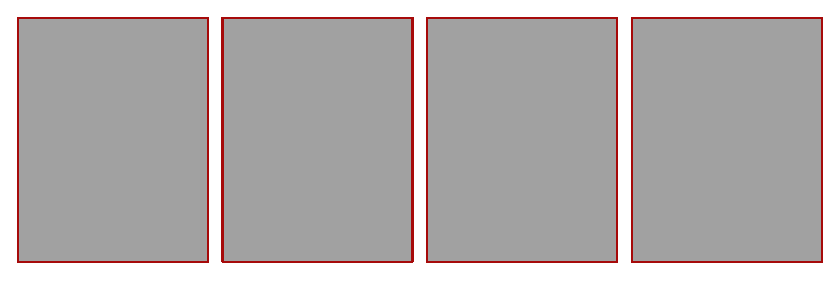
\includegraphics[width=0.7\textwidth]{comparison_ana_numa.eps}